A flight phase is defined as a mission segment of the rocket's trajectory, bounded by guidance objectives and an unchanged vehicle configuration and active actuators. Considering a two stage launcher with a reusable first stage, the launch vehicles starts ascending vertically upwards for a short distance to clear the launch tower, then a pitch over manoeuvrer is performed to build the horizontal velocity for orbital insertion. This phase, called the \textit{gravity turn} ascends the launcher through dense atmospheric layers having to throttle its engines to avoid reaching the maximum dynamic pressure limit. For Space X missions this is commonly seen at 30-35 kPa. Furthermore, the high dynamic pressure causes aerodynamic disturbances to be larger motivating a small angle of attack which can be achieved through an aerodynamically stable rocket. Aerodynamic stability requires the center of pressure to be aft of the center of gravity so an increase in the absolute angle of attack provides a counteracting moment.


To perform the pitch over the launch vehicle uses thrust vectored control of its engines to enact a force perpendicular to the rocket forcing the flight path angle to decrease and hence the pitch angle as the angle of attack self-corrects. When the propellant assigned for the first stage burn is consumed the rocket will perform \textit{stage separation}. The second stage will burn to put it on a ballistic arc trajectory to its desired orbit before a circularisation burn occurs.

The first stage, after separation, starts the descent procedure. Two options for vertical landing are present, first a Return To Launch Site (RTLS) scenario where the rocket returns to a landing pad nearby or the actual launch tower. Second is the Away From Launch Site (AFLS) landing on a landing pad downrange, Space X performs this by landing on an autonomous drone-ship. RTLS has lower operation costs as no drone ship or secondary landing pad is required. Furthermore, as it is directly at the launch site it allows for quicker refurbishment, key for higher frequency rocket launch. AFLS uses less fuel as horizontal velocity increment for landing is less allowing for increased payload capacity. However, for an ocean landing it is dependent on ocean conditions, restricting launch windows. As a result, RTLS is the chosen scenario as it will provide a higher frequency of launchs, increasing access to space.

A \textit{flip-over manoeuvrer} is performed through thrust vectored control on a limited amount of engines to orientate the rocket horizontally facing towards the landing site. Once horizontal, this engines continue burn in a phase called the \textit{boostback burn} to provide a horizontal thrust to take the stage to desired horizontal velocity reference to place to place it on a ballistic arc path back to the launch site. Excess ullage gas is occurrent during boostback burn as the main tank is near empty from the ascent burn leaving an expanded pressurant which is used by cold gas thrusters in the reaction control system's cold gas thrusters to provide fine attitude control in the upper atmosphere where actuated aerodynamic control surfaces are ineffective due to a low dynamic pressure.

The \textit{high altitude ballistic arc} starts with the stage coasting to its apogee before descending, with the cold gas thrusters used in this example to provide attitude control. The aim is to orientate the rocket to have a zero effective angle of attack, the angle of attack with regards to the a flipped rocket.

The \textit{powered descent phase} occurs, here two options are present first a separated \textit{re-entry burn} followed by a \textit{low altitude ballistic arc} and finally a \textit{landing burn}. The RETALT project, an EU-funded project to develop and validate technologies for reusable vertical-landing launch vehicles, \cite{dezaiacomo2022retalt} followed this sceanairo. The motivation for each phase is shown below, and the mission profile is depicted in \autoref{fig:RETALT1_flightplant}.
\begin{itemize}
    \item Re-entry burn: manage the velocity to maintain the aero-thermal-mechanical loads present on the vehicle after the ballistic arc. These loads occur from high dynamic pressure, aerodynamic heating and structural stresses. The rocket has a maximum dynamic pressure defined as 100kPa and a maximum g-load as 2.5.
    \item Low altitude ballistic arc: slows the stage down while providing trajectory correction from uncertainties in previous flight phases and this ballistic arc. The desired outcome is to slow the vehicle to meet set initial conditions for the landing burn.
    \item Landing burn: aims to precisely land the stage on the landing pad with a zero touchdown velocity.
\end{itemize}

\begin{figure}[h!]
    \centering
    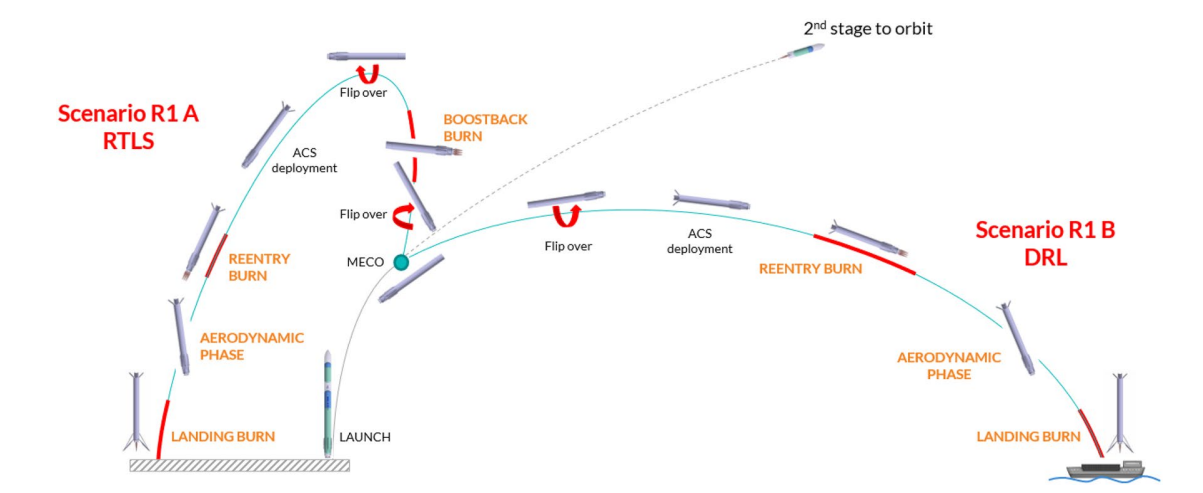
\includegraphics[width=0.95\linewidth]{Figures/RETALT1landing.png}
    \caption{RETALT1 return mission concept (\cite{dezaiacomo2022retalt})}
    \label{fig:RETALT1_flightplant}
\end{figure}

The Falcon 9 rocket performs this split burn sceanairo, heavier the new Super Heavy booster performs a single burn, as its design can handle the aero-thermal-mechanical loads present during re-entry. CALLISTO, a joint project from CNES, DLR and JAXA space agencies, to develop a smal reusable vertical take-off and landing rocket, fly to 40km and decend with a maximum dynamic pressure limit of under 35 kPa shown in their trajectory \cite{Desmariaux2019CALLISTO}.

The high dynamic pressure requires a low effective angle of attack, as the aerodynamic forces acting on the body are proportional to dynamic pressure and effective angle of attack. Areas of high dynamic pressure also increase the control authority of movable Aerodynamic Control Surfaces (ACS), like grid fins, as such they can provide orientation control. As a dynamic pressure decreases due to low velocities just above landing, TVC takes over orientation control.